% kapitel2.tex
\chapter{Definitionen}
\label{cha:definitionen}

Vorab werden einige Definitionen und Notationen festgelegt, die im Verlauf der Arbeit verwendet werden.
Der Algorithmus arbeitet mit einem ungerichteten Graph $G = (V, E)$ ohne Mehrfachkanten, wobei $E$ die Menge der Kanten und $V$ die Knotenmenge sei.
\begin{wrapfigure}{r}{6cm}
  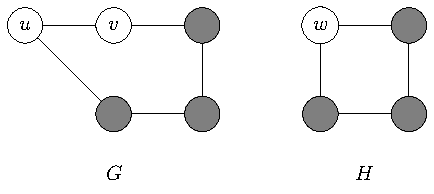
\includegraphics[width=6cm]{bilder/Kantenkontraktion.pdf}
  \caption{Die Kante, die $u$ und $v$ in $G$ verbindet, wird kontrahiert, sodass sie in $H$ durch den neuen Knoten $w$ ersetzt wird.}
  \label{fig:Kantenkontraktion}
\end{wrapfigure}
Eine Kante $e \in E$, die zwei Knoten $u$ und $v$ verbindet, wird durch $e = (u, v)$ angegeben.
Ein Pfad $P(u, v)$ verbindet zwei Knoten $u$ und $v$ über eine Folge von Knoten, die adjazent zueinander sind.
Bei der Kontraktion einer Kante $e = (u, v)$ wird diese mit ihren beiden Endpunkten aus dem Graph entfernt und einen neuen Knoten $w$ ersetzt.
Die Nachbarknoten von $w$ werden auf die Menge der adjazenten Knoten von $u$ und $v$ gesetzt.
In Abbildung \ref{fig:Kantenkontraktion} ist das Vorgehen skizziert.
Analog kann, wie in Abbildung \ref{fig:Pfadkontraktion} gezeigt, ein Pfad kontrahiert werden, wobei der neu eingefügte Knoten $w$ Kanten zu der Menge der adjazenten Knoten aller Knoten des Pfades besitzt.
\begin{wrapfigure}{l}{6cm}
  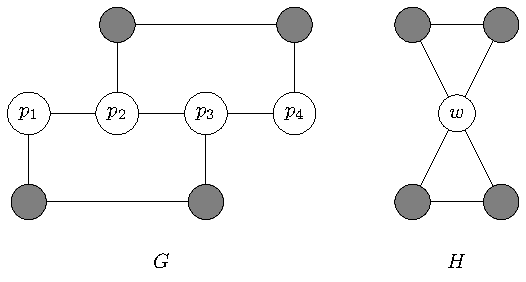
\includegraphics[width=6cm]{bilder/Pfadkontraktion.pdf}
  \caption{Der Pfad von $p_1$ bis $p_4$ wird kontrahiert.
           Der neue Knoten $w$ in $H$ enthält alle Nachbarn der Pfadknoten in $G$.}
  \label{fig:Pfadkontraktion}
\end{wrapfigure}

Ein Minor $H$ eines Graphen $G$ bezeichnet einen Graph, der isomorph zu $G$ ist, nachdem eine beliebige Menge an Operationen von Kantenkontraktionen, Kantenentfernungen und Knotenentfernungen durchgeführt wurde.
Ein Beispiel dazu findet sich in Abbildung \ref{fig:Minor}.
Jeder Graph ist sein eigener Minor, genauso ist jeder Teilgraph ein gültiger Minor.
Dass $H$ ein Minor von $G$ ist, wird dargestellt durch $H$ \minor $G$.
Das Branch-Set eines Knotens $w$ aus einem Minor von $G$ bezeichnet die Menge an Knoten, die durch Kontraktionen zu $w$ verschmolzen wurden.
In Abbildung \ref{fig:Minor} besteht beispielsweise das Branch-Set von $g$ aus $\{a, b, c\}$, zu $f$ in $H_2$ gehört die Knotenmenge $\{f\}$ in $G$.
Für die Knotenmenge $U \in V$ bezeichnet $G \setminus U$ den Teilgraph, der entsteht, wenn alle Knoten aus $U$ mit ihren inzidenten Kanten aus $G$ entfernt werden.
Ein Homöomorph eines Graphen $G$ enthält alle Knoten und Kanten aus $G$, zusätzlich können aber Kanten als gegenteilige Operation zur Kontraktion unterteilt werden.
Für eine Kante $e = (u, v)$ bedeute das, dass $e$ entfernt wird, dafür ein neuer Knoten $w$ und zwei neue Kanten $(u, w)$ und $(w, v)$ eingefügt werden.
\begin{figure}[H]
  \centering
  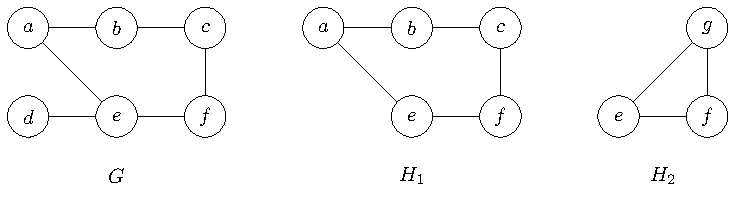
\includegraphics[keepaspectratio]{bilder/Minor.pdf}
  \caption{Ein Graph $G$ mit seinen Minoren $H_1$ und $H_2$.
           Um $H_1$ zu erhalten, wurde in $G$ die Kante $(d, e)$ und anschließend der Knoten $d$ entfernt.
           Für $H_2$ wurden außerdem der Pfad $P(a, c)$ kontrahiert.}
  \label{fig:Minor}
\end{figure}

\begin{wrapfigure}{r}{4cm}
  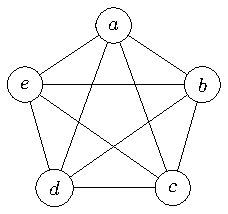
\includegraphics[width=4cm]{bilder/K_5.pdf}
  \caption{Der Graph \kf.}
  \label{fig:K5}
\end{wrapfigure}
Ein Graph wird als planar bezeichnet, wenn er sich so in der Ebene einbetten lässt, dass sich keine Kanten kreuzen.
Ein \kf (\sAbb \ref{fig:K5}) ist ein spezieller Graph, der aus fünf Knoten besteht, die alle zueinander adjazent sind.
Ein \kdd (\sAbb \ref{fig:K33}) ist ein vollständig bipartiter Graph mit sechs Knoten.
Er lässt sich also in zwei Knotenmengen unterteilen (im Folgenden als rote und blaue Menge bezeichnet), sodass alle Knoten der einen Menge zu allen Knoten der anderen Menge benachbart sind.
Nach dem Satz von Kuratowski ist ein Graph planar, wenn er kein \kf- oder \kdd-Homöomorph als Teilgraph beinhaltet.
Eine alternative Formulierung von Wagner sagt aus, dass ein Graph planar ist, wenn er keinen \kf-Minor oder \kdd-Minor enthält.\cite{Die12}
\begin{wrapfigure}{r}{4cm}
  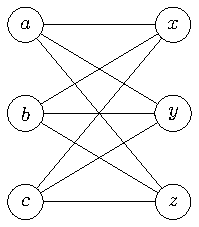
\includegraphics[width=4cm]{bilder/K_33.pdf}
  \caption{Der Graph \kdd.}
  \label{fig:K33}
\end{wrapfigure}

Als nächstes wird ein \kdd genauer betrachtet.
Sei dessen rote Knotenmenge $R = \{a, b, c\}$ und blaue $B = \{x, y, z\}$
Diese sechs Knoten werden in einem \kdd-Homöomorph $H$ als Branch-Ends genannt und zeichnen sich dadurch aus, dass sie als einzige Knoten in $H$ den Grad 3 haben.
Ein Branch-Path in $H$ ist ein Pfad, der zwei Branch-Ends verbindet, beispielsweise $P(a, x)$.
Ein Branch-Fan bezieht sich immer auf einen der Branch-Ends und wird \zB für $a$ als $F(a)$ geschrieben.
Bezeichnet werden dadurch alle Pfade, die zu einem anderen Branch-End führen - für $a$ also die Pfade $P(a, x)$, $P(a, y)$ und $P(a, z)$.


Der Graph $W$ bezeichnet einen speziellen Graph, der aus acht Knoten besteht.
Seine äußeren Kanten bilden einen Kreis, außerdem sind die Knoten jeweils adjazent zu den gegenüberliegenden. Eine Darstellung findet sich links in Abbildung \ref{fig:W}.
Er enthält einen \kdd als Minor (in der Abbildung rechts angedeutet), jedoch keinen \kf.
Als $M$ wird ein Graph bezeichnet, der einen \kdd als Teilgraph enthält, jedoch einen zusätzlichen Knoten und zwei zusätzliche Kanten enthält.
Er ist insofern interessant, als dass er, wie in Abbildung \ref{fig:M} zu sehen, neben einem \kdd-Minor auch einen \kf-Minor enthält.
\begin{figure}[H]
  \centering
  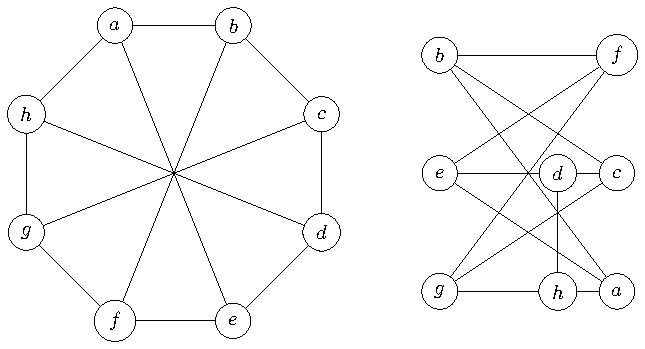
\includegraphics[keepaspectratio]{bilder/W.pdf}
  \caption{Der Graph $W$, links in seiner üblichen Darstellung, rechts mit angedeutetem \kdd-Minor.}
  \label{fig:W}
\end{figure}

\begin{figure}[H]
  \centering
  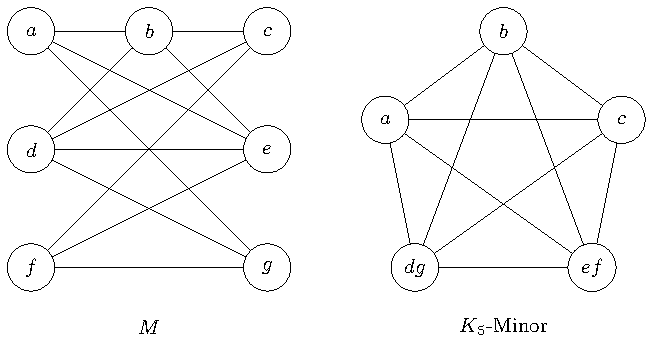
\includegraphics[keepaspectratio]{bilder/M.pdf}
  \caption{Der Graph $M$ sowie ein \kf-Minor aus $M$.}
  \label{fig:W}
\end{figure}

Als $(i)$-Separator wird eine Menge $S$ bestehend aus $i$ Knoten in einem zusammenhängenden Graph $G$ bezeichnet, sodass $G \setminus S$ nicht mehr zusammenhängend ist.
Ein $(i, j)$-Separator ist ein $i$-Separator, sodass $G-S$ aus mindestens $j$ Zusammenhangskomponenten besteht.
In Abbildung \ref{fig:AugmentierteKomponenten} wird ein \dd-Separator im linken Graph gezeigt.
Durch einen Separator können augmentierte Komponenten definiert werden:
Sind $C \in V$ die $i$ Knoten, die zu einem $(i, j)$-Separator in $G$ gehören, wird der Graph durch $G \setminus C$ zunächst in $j$ Zusammenhangskomponenten zerlegt.
Anschließend werden Kopien der Knoten aus $C$ zu jeder Komponente hinzugefügt.
Sie bilden dabei in jeder Zusammenhangskomponente eine Clique.
Außerdem besitzen sie Kanten zu Knoten in der Zusammenhangskomponente, falls eine Kante $e = (c, z)$ in $G$ existierte, $c \in C$ und $z$ ein Knoten der Zusammenhangskomponente ist.
Jeder der resultierenden Graphen ist eine augmentierte Komponente des Urpsrungsgraphen $G$ und wie in Theorem \ref{Theorem33} bewiesen wird, \evtl ein Minor zu $G$.
Als gegenteilige Operation kann eine Cliquen-Summe verwendet werden, um zwei Graphen zu verschmelzen.
Dazu müssen zwei Graphen $H_1$ und $H_2$ als Teilgraph eine gleich große Clique enthalten.
$H_1$ und $H_2$ können zu einem Graph zusammengefügt werden, indem je ein Knoten von der Clique in $H_1$ und in $H_2$ zu einem zusammengefügt werden.
Im resultiernden Graph dürfen außerdem Kanten zwischen den Knoten der Clique entfernt werden.
Dadurch ist es möglich, einen Graph $G$ in augmentierte Komponente zu zerlegen und anschließend durch eine Cliquen-Summe wieder $G$ zu erhalten.
Dieses Vorgehen wird in Abbildung \ref{fig:AugmentierteKomponenten} gezeigt, dabei wird der linke Graph rechts in augmentierte Komponenten zerlegt \bzw von rechts nach links werden drei Graphen durch eine Cliquen-Summe zusammengefügt.
\begin{figure}[H]
  \centering
  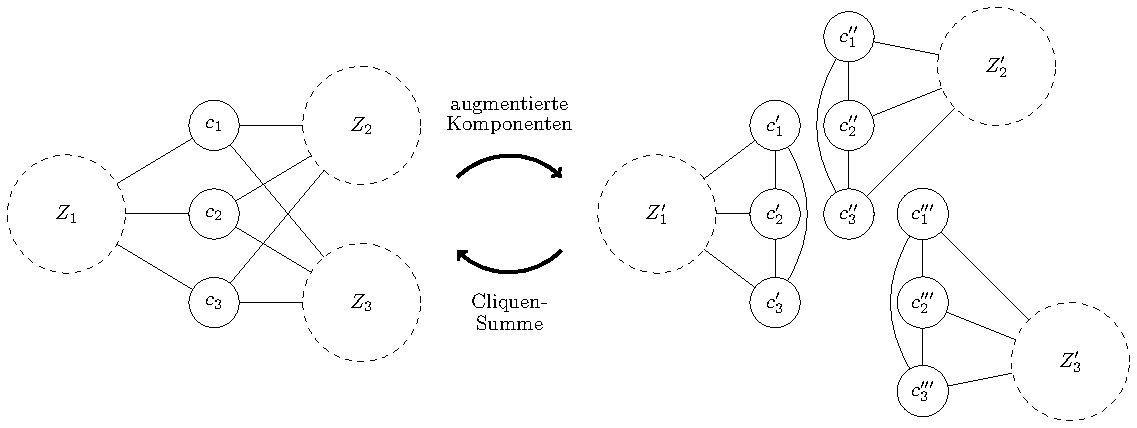
\includegraphics[keepaspectratio]{bilder/Augmentierte_Komponenten.pdf}
  \caption{Der linke Graph wird in drei augmentierte Komponenten durch den \dd-Separator $C = \{c_1, c_2, c_3\}$ geteilt.
           Alle $Z_i$ und $Z_i'$ stellen Teilgraphen dar, die zur Übersicht zu einem Knoten zusammengefügt wurden.
           Die drei rechten Graphen können durch die Cliquen-Summe der Cliquen $\{c_1', c_2', c_3'\}$ sowie $\{c_1'', c_2'', c_3''\}$ und $\{c_1''', c_2''', c_3'''\}$ den rechten Graph erzeugen.
           Während der Cliquen-Summen Operation dürfen die Kanten, die die Knoten in den Cliquen verbinden, gelöscht werden.}
  \label{fig:AugmentierteKomponenten}
\end{figure}
